\documentclass{beamer}
\usepackage[utf8]{inputenc}
\usepackage[MeX]{polski}
\usepackage{graphicx}
\usepackage{listings}
\usepackage{array}
\usepackage{xcolor}
\usepackage{colortbl}
\usepackage{subfig}
\usetheme{Warsaw}
\usecolortheme[rgb={0,0.5,1}]{structure}
\setbeamerfont{title}{family=\rm}
\setbeamerfont{author}{family=\it}
\title{Problem plecakowy}
\subtitle{Projektowanie algorytmów i metod sztucznej inteligencji}
\author{Michał Wieczorek, Artur Szafraniak}
\institute{
Automatyka i Robotyka,
Wydział Elektroniki\\
Politechnika Wrocławska}

\begin{document}
\begin{frame}
\titlepage
\end{frame}

\section{Spis treści}
\begin{frame}
	\frametitle{Plan prezentacji}
	\tableofcontents
\end{frame}

\section{Wprowadzenie}
\subsection{Opis problemu}
\begin{frame}
	\frametitle{Opis problemu}
	\begin{figure}[H]
	\centering
	
\includegraphics[scale=0.3]{zlodziej2.png}
	\end{figure}
\end{frame}

\section{Sposoby rozwiązania}
\subsection{Algorytmy zachłanne}
\begin{frame}
	\frametitle{Rodzaje algorytmów zachłannych}
	\begin{itemize}
	\item Sortowanie według wartości towaru\\
		$c_{1} \leq c_{2} \leq c_{3} \leq \ ... \leq c_{n}$
	\item Sortowanie według objętości\\
		$m_{1} \geq m_{2} \geq m_{3} \leq \ ... \geq m_{n}$
	\item Sortowanie według współczynnika wartość/objętość\\
		$\dfrac{c_{1}}{m_{1}} \leq \dfrac{c_{2}}{m_{2}} \leq \dfrac{c_{3}}{m_{3}} \leq \ ... \leq \dfrac{c_{n}}{m_{n}}$
	\end{itemize}
\end{frame}

\subsection{Algorytm Knapsack 0-1}
\begin{frame}[fragile]
	\frametitle{Algorytm \textit{Knapsack 0-1}}
	\begin{lstlisting}[basicstyle=\tiny,tabsize=2]
void Magazyn::knapsack(int wielkosc) {
	int i, j; // pomocnicze liczniki
	int tmp[ROZMIAR + 1][wielkosc + 1]; // tablica pomocnicza do przechowywania danych

	for (i = 0; i <= ROZMIAR; i++) {
		for (j = 0; j <= wielkosc; j++) {
			if (i == 0 || j == 0) { // zerowe indeksy wypelniamy zerami
				tmp[i][j] = 0;
			}
			else if (tab[i].get_masa() <= j) {
				// znalezienie maksimum
				tmp[i][j] = max(
						tab[i].get_wartosc()
								+ tmp[i - 1][j - tab[i].get_masa()],
						tmp[i - 1][j]);
			}
			else { // zwykle przepisanie z wyzszego indeksu tablicy
				tmp[i][j] = tmp[i - 1][j];
			}
		}
	}
	\end{lstlisting}
\end{frame}

\begin{frame}
	\frametitle{Przykład}
\begin{table}[]
\begin{tabular}{|c|c|c|}
\hline
Nazwa        & Waga & Wartość	\\ \hline
\alt<3-7>{\color{blue}Kolczyki}{\color{black}Kolczyki} & \alt<3-7>{\color{blue}3}{\color{black}3} &
\alt<3-7>{\color{blue}100}{\color{black}100} 	\\ \hline
\alt<8-12>{\color{blue}Pierscionek}{\color{black}Pierscionek} & \alt<8-12>{\color{blue}2}{\color{black}2} & 
\alt<8-12>{\color{blue}20}{\color{black}20} 	\\ \hline
\alt<13-17>{\color{blue}Naszyjnik}{\color{black}Naszyjnik} & \alt<13-17>{\color{blue}4}{\color{black}4} & 
\alt<13-17>{\color{blue}60}{\color{black}60} 	\\ \hline
\alt<18-22>{\color{blue}Zegarek}{\color{black}Zegarek} & \alt<18-22>{\color{blue}1}{\color{black}1} & 
\alt<18-22>{\color{blue}40}{\color{black}40}	\\ \hline
\end{tabular}
\end{table}
\begin{table}[]
\begin{tabular}{|c|c|c|c|c|c|c|}
\hline
tmp{[}i,j{]} & j=0 & 1 & 2 & 3 & 4 & 5 \\ \hline
i=0        & \onslide<2->{0} & \onslide<2->{0} & \onslide<2->{0} &\onslide<2->{0} & \onslide<2->{0} & \onslide<2->{0}   \\ \hline
1          & \onslide<2->{0} & \onslide<3->{0} & \onslide<4->{0} & \onslide<5->{100} & \onslide<6->{100} & \onslide<7->{100} \\ \hline
2         & \onslide<2->{0} & \onslide<8->{0} & \onslide<9->{20} & \onslide<10->{100} & \onslide<11->{100} & \onslide<12->{120} \\ \hline
3          & \onslide<2->{0} & \onslide<13->{0} & \onslide<14->{20} & \onslide<15->{100} & \onslide<16->{100} & \onslide<17->{120} \\ \hline
4          & \onslide<2->{0} & \onslide<18->{40} & \onslide<19->{40} & \onslide<20->{100} & \onslide<21->{140} & \onslide<22->{140} \\ \hline
\end{tabular}
\end{table}
\end{frame}

\subsection{Wybieranie elementów do plecaka}
\begin{frame}[fragile]
\frametitle{Wybieranie elementów do plecaka}
\begin{lstlisting}[basicstyle=\small, tabsize=2]
	i = ROZMIAR;
	j = wielkosc;

	while (i > 0 && j > 0) {
		if (tmp[i][j] != tmp[i - 1][j]) {
			plecak.push_back(tab[i]);
			j = j - tab[i].get_masa();
			i = i - 1;
		}
		else {
			i = i - 1;
		}
	}
	
\end{lstlisting}
\end{frame}

\begin{frame}
	\frametitle{Przykład }
\begin{table}[]
\begin{tabular}{|c|c|c|}
\hline
Nazwa        & Waga & Wartość	\\ \hline
\alt<11->{\cellcolor{green}Kolczyki}{\color{black}Kolczyki}     & \alt<12->{\color{blue}3}{\color{black}3} 	&  100 	\\ \hline
Pierościonek & 2    & 20 	\\ \hline
Naszyjnik    & 4    & 60 	\\ \hline
\alt<3->{\cellcolor{green}Zegarek}{\color{black}Zegarek} & 
\alt<4>{\color{blue}1}{\color{black}1} & 40 	\\ \hline
\end{tabular}
\end{table}
\begin{table}[]
\begin{tabular}{|c|c|c|c|c|c|c|}
\hline
tmp{[}i,j{]} & j=0 & 1 & 2 & 3 & 4 & 5 \\ \hline
i=0        & \alt<13->{\color{blue}0}{\color{black}0} & 0 & 0 & 0 & \alt<10-12>{\color{red}0}{\color{black}0} & 0  \\ \hline
1          & 0 & 0 & 0 & 100 & \alt<8-12>{\color{blue}100}{\color{black}100} & 100  \\ \hline
2          & 0 & 0 & 20 & 100 & \alt<6-8>{\color{red}100}{\color{black}100} & 120  \\ \hline
3          & 0 & 0 & 20 & 100 & \alt<5-6>{\color{blue}100}{\color{black}100} & \alt<2-4>{\color{red}120}{\color{black}120}  \\ \hline
4          & 0 & 40 & 40 & 100 & 140 & \alt<1-4>{\color{blue}140}{\color{black}140}  \\ \hline
\end{tabular}
\end{table}
\end{frame}

\begin{frame}
\frametitle{Przykład }
Ostatecznie w plecaku znalazły się:

\begin{figure}
\subfloat[Kolczyki \label{fig:1}]{
    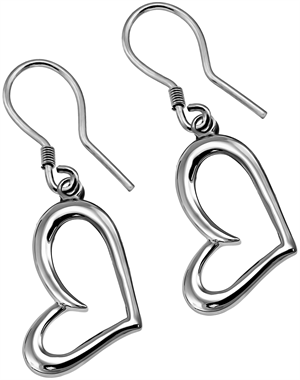
\includegraphics[width=0.25\textwidth]{kolczyki.png}}
\subfloat[Zegarek \label{fig:2}]{
    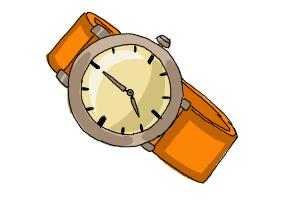
\includegraphics[width=0.45\textwidth]{zegarek.png}}
\end{figure}

\end{frame}
\begin{frame}
\centering
\frametitle{Zakończenie}
Dziękujemy za uwagę :)
\end{frame}
\end{document}